\documentclass[12pt, a4paper]{article}
\usepackage[ddmmyyyy]{datetime}
\usepackage{graphicx}
\renewcommand{\figurename}{Şekil}
\renewcommand{\refname}{Kaynaça}
\graphicspath{{images/}}
\renewcommand{\dateseparator}{.}
\usepackage{caption}
\usepackage{subcaption}
%\usepackage{natbib}
\usepackage{pdflscape}
\begin{document}

\title{\textbf { T.C Kütahya Sağlık Bilimleri Üniversitesi}}
\begin{figure}
	\centering
	
\includegraphics[width=7 cm  ,height=6 cm  ]{logo.jpg}
	


\end{figure}
\author{Motion Capture 3D: Gerçek Zamanlı Hareket Yakalama \\ \\  Ders Sorumlusu:Emre Güngör \\  İlknur Koparır 2118121010  }

\date{\today}

\maketitle
\begin{figure}
	\centering
	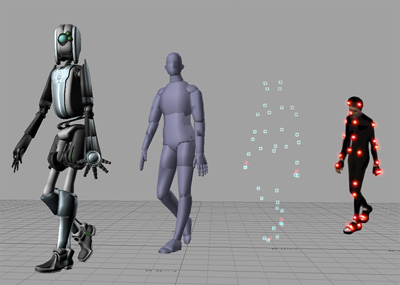
\includegraphics[width=15 cm  ,height= 5 cm  ]{Activemarker2.png}
	
\end{figure}

\newpage


\section{Giriş}  Hareket yakalama teknolojisi (motion capture), yüzyılı aşkın bir süre içerisinde
insanlığın geliştirdiği teknolojinin etkileri ile büyük ölçüde gelişim göstermiştir.
Günümüzde sanat, eğlence ve teknoloji dünyasında önemli bir yere sahip olan motion capture,insanların gerçek dünyadaki hareketleri dijital ortama aktarma ihtiyacından doğmuştur.Özellikle sinema, video oyunları,
reklam endüstrisi gibi alanlarda, gerçekçi hareketlerin oluşturulması ve karakterlerin doğal bir şekilde davranması büyük bir talep görmesinden dolayı bu teknolojilerin kullanım alanları gelişmektedir.Hareket halindeki bir obje veya bir canlının üç boyutlu koordinat ve açısal değişimlerinin çeşitli yöntemlerle
bir alıcıya iletilmesi olarak tanımlanan hareket yakalama teknolojisi  \cite{ozkiricscci2022motion}, işaretleyici tabanlı ve işaretleyici tabanlı olmayan sistemler
olarak ikiye ayrılmıştır. İşaret tabanlı hareket yakalama sistemleri manyetik veya optik vericilerin insan vücudunun önemli eklem bölgelerine yerleştirilerek hareket bilgisinin üretilmesidir. İşaret tabanlı olmayan hareket tanıma sistemlerde ise verici doğrudan figür olarak karşımıza çıkmaktadır.Kameralar, insan formunu arka plandan ayrıt eden algoritmalar ve derin öğrenme teknikleri sayesinde verilerden hareket bilgisi çıkarılmaktadır.Bu teknolojiler sayesinde  daha hızlı ve hassas hareket yakalama sistemleri geliştirilerek, gerçek zamanlı etkileşimli uygulamaların performansı artırılmakta ve kullanıcı deneyimi iyileştirilmektedir.\\
 

\begin{figure}[h!]
	\centering
	\begin{subfigure}[b]{0.4\linewidth}
		\includegraphics[width=5 cm, height=5 cm]{işaretTabanli.png}
		\caption{Manyetik hareket yakalama sistemi.}
	\end{subfigure}
	\begin{subfigure}[b]{0.4\linewidth}
		\includegraphics[width=5 cm , height=5 cm]{işaretTabanliOlmayan.png}
		\caption{İşaretleyici tabanlı olmayan hareket yakalama sistemi.}
	\end{subfigure}

\end{figure}


\newpage
\section{Literatür Taraması}

Motion capture teknolojisinin kökenleri, eski çağlardan başlayarak, insanların hareketlerini taklit etme ve canlandırma ihtiyacıyla başlamıştır.

1906’da Amerikalı mucit Thomas Edison’un yardımı ile Amerikan gazetesi karikatüristi
James Stuart Blacton’un, Şekil \ref{fig:boat1}'de görüldüğü üzere ilk çizgi filmi olan Humorous Phases Faces’i (Komik Yüzlerin Mizahi
Evreleri) gösterime girmiştir.Çizgi filmde, kara tahta üzerinde, bir şapka ile oynayan palyaço ve çemberden atlayan bir köpek de dahil olmak üzere, elle çizilmiş karakterler bulunmaktaydı. Hareket ettirip durdurma tekniği kullanılan filmde, çizimler kendi başlarına tamamlanıyor ve sonra hareket eden çizimler gibi görünmekteydi. Bu teknik izleyiciler tarafından komik bulunmuş ve ilgi ile karşılanmıştır \cite{erdem2021sanali}

\begin{figure}[!h]
	\centering
	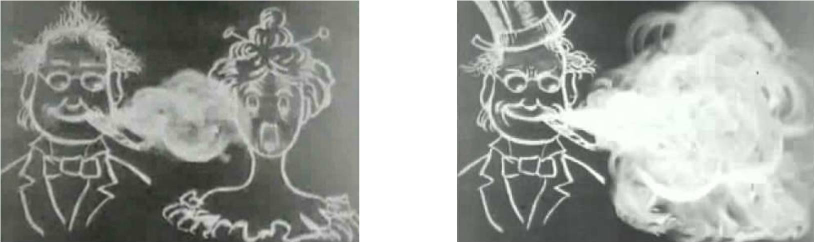
\includegraphics[width=10 cm , height = 3 cm ]{film.png}
	\caption{Humorous Phases Faces}
	\label{fig:boat1}
\end{figure}


1959’da Harrison, potansiyometrelerle (ayarlanabilir
dirençler) donatılmış bir elbiseyi oyuncuya giydirmiş ve oyuncunun tüm hareketlerini bir ekran
yardımı ile gerçek zamanlı olarak kaydetmeyi başarmıştır. Bu ilkel bir teçhizattı ancak gerçek
zamanlı hareket yakalamanın ilk örneğidir. 1980’lere gelindiğinde animatörler,
oyuncuların hareketlerini izlemek için aktif işaretçilerle kaplı vücut giysileri ve avuç
büyüklüğünde kameralar kullanmışlardır \cite{erdem2021sanali}. \\

 Teknolojinin gelişmesiyle birlikte Rosales ve ark. \cite{rosalesestimating}, kalibre edilmemiş birden fazla görüş kullanılarak 3B eklemli duruşun (pose) tahmini için bir çerçeve sunar. Bu çerçevede, Uzmanlaştırılmış Haritalama Mimarisi (SMA) adı verilen istatistiksel bir çıkarım yöntemi kullanılır. SMA, kareler ve görünümler arasında 2B eklem konumları sağlar.\\

Kakadiaris ve Metaxas \cite{desmarais2021review} , dik açılı konfigürasyonlarda çoklu kamera görüntülerini kullanarak insan vücut parçalarının 3B model tabanlı izleme ve şekil tahmini için bir yöntem sunarlar. Daha sonra yaklaşımı, çoklu görüşlü video dizilerinden insan hareketinin tahmini ve buna göre animasyon dizileri oluşturmak için genişlettiler . 


\newpage
\section{Metodoloji}
Bu çalışmada, kamera üzerinden alınan insan hareketlerini 3 boyutlu olarak gösterilmesi amaçlanmıştır.Çalışma kapsamında kameradan görüntü almak için OpenCV kütüphanesi kullanılmıştır.Vücut tespiti için ise Google tarafından geliştirilen MediaPipe framework'ü kullanılmıştır. MediaPipe, ücretsiz ve açık kaynaklı bir makine öğrenmesi framework'üdür ve içinde Object Detection, image classification ve test classification gibi birçok model barındırmaktadır.\\MediaPipe'ın Holistic yöntemi, aynı anda yüz, el ve vücut pozisyonlarının  takibini mümkün kılmaktadır.Bu yöntem, Şekil \ref{fig:mesh1}'de görülebileceği üzere tek bir kare üzerinden 33 noktanın tespit edilmesine izin verirken, geleneksel COCO topolojisinde tek bir kare üzerinde 17 noktanın tespit edilmesini mümkün kılmaktadır.Bu yöntemle, 33 poz, 21 el ve 468 yüz işaret noktası olmak üzere toplamda 543 işaret noktası tespit edilebilir. Mobil cihazlarda bile gerçek zamanlı çalışabilmektedir.Holistic yöntemi çalışırken ilk olarak poz tespiti yapılır, ardından tespit edilen poz işaret noktalarından yola çıkılarak da eller ve yüz bölgesi saptanıp o bölümler ayrıca işaretlenir. En son olarak bulunan tüm noktalar birleştirilir.Böylece vücut tespiti yapılmış olup ilerleyen aşamalarda, MediaPipe ile tespit edilen landmark'lerin bvh dosyasına kaydedilmesi ve bu dosyanın Unreal'da 3 boyutlu bir karaktere uygulanması amaçlanmaktadır. Karakterler öncelikle  çevrimiçi ve mocap animasyon veritabanı olan  Mixamo'dan fbx formatında indirilip ve daha sonra Unreal ortamına aktarılacaktır.



\begin{figure}[h]
	\centering
	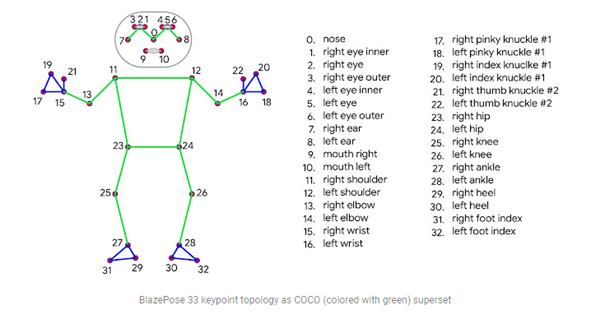
\includegraphics[width=1.0\textwidth]{pose_landmarks.png}
	\caption{MediaPipe'da 33 vücut parçasının konumu}
	\label{fig:mesh1}
\end{figure}



\newpage
\begin{landscape}
\subsection{Sistem Tasarımı}

	\begin{figure}[!htbp] %[h]
		\caption{GANTT CHART}
		\centering
		%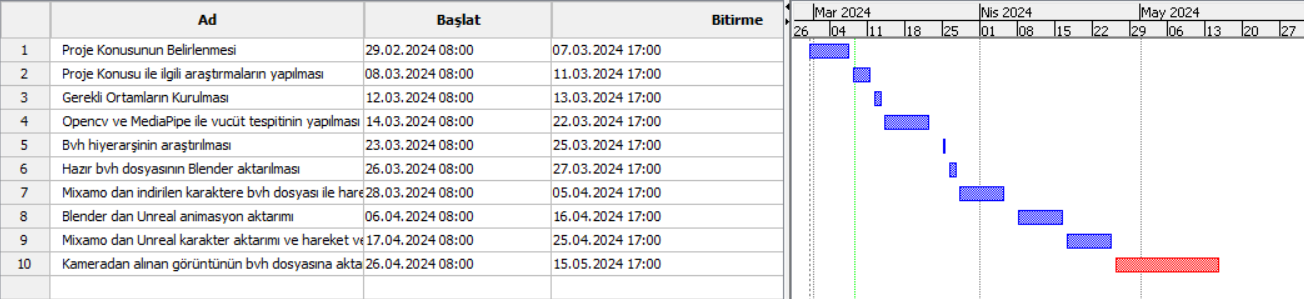
\includegraphics[angle=90, width=\textwidth]{x.png}
		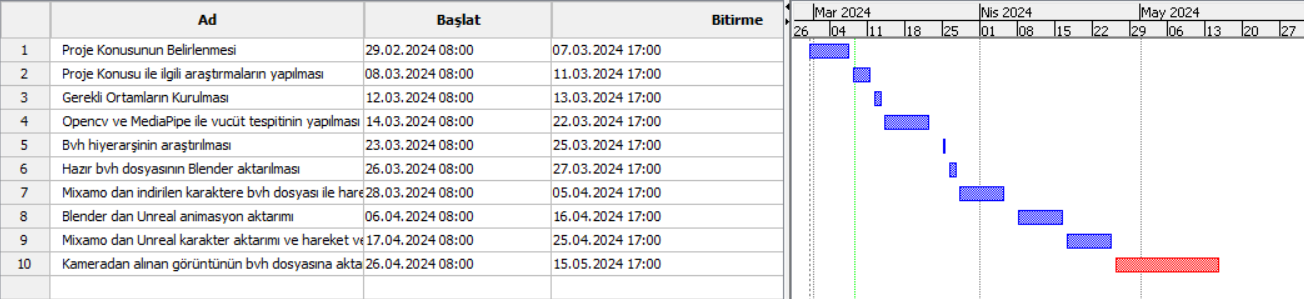
\includegraphics[height= 5 cm]{x.png}
		\label{gantt}
	\end{figure}
\end{landscape}
\newpage
\section{Beklenen Sonuçlar}
Hareket yakalama teknolojisi son yıllarda biyomekanik, yaya
navigasyonu, eğitim ve simülasyon, sanal gerçeklik ve
karakter animasyonu alanlarında oldukça önem kazanmıştır.
Bu çalışmada da kameradan alınan görüntüdeki hareketlerin tespit edilip bu hareketlerin 3 boyutlu olarak unreal ortamına aktarılması amaçlanmaktadır.

\bibliographystyle{ieeetr}
\bibliography{references}
 

\end{document}